\documentclass[a4paper,10pt]{article}
%\documentclass[a4paper,10pt]{scrartcl}
%\documentclass[3p,times]{elsarticle}
\usepackage[utf8]{inputenc}

% Pretty much all of the ams maths packages
\usepackage{amsmath,amsthm,amssymb,amsfonts}

% Typesets URLs sensibly - with tt font, clickable in PDFs, and not breaking across lines
\usepackage{url}
\usepackage{graphicx}
\usepackage[english]{babel} % bilingua 


\usepackage[usenames,dvipsnames]{color}
\title{Gaussian Mixture Model with MapReduce}% o using Hadoop o quello che
\author{Andrea Mannocci, Giuseppe Portaluri, Lucia Vadicamo}
\date{}

\pdfinfo{%
  /Title    (Gaussian Mixture Model with MapReduce) %EM for Gaussian Mixtures using MapReduce 
  /Author   (Andrea Mannocci, Giuseppe Portaluri,Lucia )
}


%\newcommand{\bb}[1]{\boldsymbol {#1}} %\textbf{}
%\newcommand{\bx}{\boldsymbol {x}} 
%\newcommand{\bw}{\boldsymbol {w}} 
%\newcommand{\bm}{\boldsymbol {\mu}} 
%\newcommand{\bs}{\boldsymbol {\sigma}} 
%\newcommand{\LX}{\mathcal{L}(X|\lambda)} 
\begin{document}
\maketitle
Suppose we have a dataset of observations $X=\{x_1, \dots, x_n\}$, $x_j\in \mathbb{R}^d$, and we wish to model this data using a mixture of Gaussians. We can estimate the parameters of a Gaussian Mixture Model (GMM) using the Expectation-Maximization (EM) algorithm \cite{bishop06} to optimize a Maximum Likelihood (ML) criterion.
We denote the parameters of a $k$-component GMM by $\Theta=\{w_i \in \mathbb{R}, \mu_{i}\in\mathbb{R}^d, \Sigma_i \in \mathbb{R}^{d\times d};\, i=1,\dots, k\}$, where $w_{i}$, $\mu_i$, $\Sigma_i$ are respectively the mixture weight, mean vector and covariance matrix of Gaussian $i$.
The Gaussian mixture distribution can be written as:
\begin{equation}
p_\Theta(x)=\sum_{i=1}^k w_i p_i(x),
\end{equation}
where
\begin{equation}
p_i(x)=\dfrac{\exp\{-\frac{1}{2}(x-\mu_i )^T\Sigma_i^{-1}(x-\mu_i )\}}{(2\pi)^{\frac{d}{2}} |\Sigma_i|^\frac{1}{2}}
\end{equation}
and 
\begin{equation}
\label{eq:constrain}
\sum_{i=1}^k w_i=1, \quad w_k\geq 0 \qquad \forall\,  i=1, \dots, k.
\end{equation}


If we assume that the data points are drawn independently from the distribution, then we can express the log of the likelihood function as:
\begin{equation}
\ln p(X| \Theta)=\sum_{s=1}^ n \ln \left\{ \sum_{i=1}^k w_i p_i(x_t|\Theta)\right\}.
\end{equation} 

%questa parte va eliminata nella relazione ed inserita nei commenti del codice%
%It is well know that ML estimation of GMM is a non-convex optimization problem for more that one Gaussian. Hence different initializations might lead to different solutions.
%Also note that some singularity can arise in the likelihood function when a single Gaussian collapses onto a specific data point (see \cite{bishop06} Section 9.2.2 for more details). Then in applying ML to GMM we must take steps to avoid finding pathological solution. A suitable heuristics  is detecting when a Gaussian component is collapsing and resetting its mean  to a randomly chosen value while also resetting its covariance to some large value, and then continuing with the optimization. 

\section{EM for Gaussian mixtures}
Given a dataset $X$ and a Gaussian Mixture Model, the goal is to maximize the likelihood function with respect to the parameters (comprising the means and covariances of the components and the mixing weight). 

\begin{enumerate}
	\item Initialize the means $\mu_i$, covariances $\Sigma_i$ and mixing coefficient $w_i$.  $K$-means algorithm can be used to find a suitable initialization.% of the GMM. 
	\item \textbf{Expectation step (E-step)} Use the current values of the current parameters to calculate the posterior probabilities $\gamma_s(i)$
	\begin{equation}
	\gamma_s(i):=p(i|x_s,\Theta)=\dfrac{w_i p_i(x_s|\Theta)}{\sum _{j=1}^k w_j  p_j(x_s|\Theta)} \qquad \forall\, i=1,\dots, k.
	\end{equation}
	\item \textbf{Maximization step (M-step)} Use the posterior probabilities $\gamma_s(i)$ to re-estimate the means, variances, and mixing coefficient:
	\begin{align}
	w_i^{\text{new}}&=\dfrac{n_i}{n}\label{eq:newParam1} \\
	\mu_i^{\text{new}}&=\dfrac{1}{n_i} \sum_{s=1}^{n} \gamma_s(i)x_s \label{eq:newParam2}\\
	\Sigma_i^{\text{new}}&= \dfrac{1}{n_i}\sum_{s=1}^{n} \gamma_s(i) (x_s-\mu_i^{\text{new}})(x_s-\mu_i^{\text{new}})^T
	%\|x_s-\mu_i^{\text{new}}\|_2^2 
	\label{eq:newParam3}
	\end{align}
	where $n_i=\sum_{s=1}^n \gamma_s(i)$, for all $i=1,\dots,k$.
	\item Check for convergence of either the parameters or the log likelihood. If the convergence criterion is not satisfied return to step 2.
\end{enumerate}

Each update to the parameters resulting from an E-step followed by an M-step is guaranteed to increase the likelihood function. The algorithm is deemed to have converged when the change in the likelihood function, or alternatively in the parameters, falls below some threshold.

In our experiments we are interested to fit a GMM on a dataset of image local features, such as SIFTs \cite{lowe99}. We assume diagonal covariances matrices and we denote $\sigma^2_i\in \mathbb{R}^d$ the variance vectors, i.e. the diagonal of $\Sigma_i$.
This is a suitable assumption for most computer vision applications, where estimating a full covariance matrix would be prohibitive due to the relative high dimensionality of the data. For example, when clustering SIFT features, each data vector has dimension 128, and each full covariance matrix would contain more than 8k distinct parameters.

Note also that the equations \ref{eq:newParam1}-\ref{eq:newParam3} can be computed in terms of the following 0-order, 1st-order and 2nd-order statistics:
%\begin{align*}
%S_0(i)&=\sum_{s=1}^n \gamma_s(i) \qquad i=1,\dots k\\
%S_1(i) &=\sum_{s=1}^n\gamma_s(i) x_s \qquad  i=1,\dots k\\
%S_2 (i) &=\sum_{s=1}^n \gamma_s(i)  x_s^2 \qquad i=1, \dots k
%\end{align*}
\begin{align*}
S_0(i)=\sum_{s=1}^n \gamma_s(i), \quad
S_1(i) =\sum_{s=1}^n\gamma_s(i) x_s, \quad
S_2 (i) =\sum_{s=1}^n \gamma_s(i)  x_s^2, \qquad i=1, \dots k
\end{align*}
where $S_0(i) \in \mathbb{R}$, $S_1(i) \in \mathbb{R}^d$ and $S_2(i) \in \mathbb{R}^d$. The square of a vector must be intended as a term-by-term operation.
We have:
\begin{align}
w_i^{\text{new}}=\dfrac{S_0(i)}{n}, \qquad
\mu_i^{\text{new}}=\dfrac{S_1(i)}{S_0(i)},  \qquad
(\sigma^2_i)^{\text{new}}=%\dfrac{(\mu_i^2)^{\text{new}} S_0(i)-2\mu_i^{\text{new}}S_1(i)+S_2(i)}{S_0(i)}=
\dfrac{S_2(i)}{S_0(i)}-\dfrac{S_1(i)^2}{S_0(i)^2} .
\end{align}

%
%For this reason, it is sometimes desirable to globally decorrelated the data before learning a GMM mode. This can be obtained by pre-multiplying the data by the inverse of a square root of its covariance.
\section{MapReduce implementation}
In our implementation of the EM algorithm for this project, each iteration is performed by a MapReduce job described as follows.

Input: a data set of observations $X=\{x_1, \dots, x_n\}$, such as the local descriptors of several images.
\begin{description}
	
	\item[{Map}]
	\textit{Key in}: -, \textit{Value in}: $ x_s\in \mathbb{R}^d$ 
	\begin{itemize}
		\item read current Gaussian parameters $\Theta=\{w_i \in \mathbb{R}, \mu_{i}\in\mathbb{R}^d, \sigma_i^2 \in \mathbb{R}^{d};\, i=1,\dots, k\}$ from HDFS.
		\item E-step: compute 	$\gamma_s(i)$, $\forall\, i=1,\dots,k$.
		\item precompute statistics:
		
		$
		\qquad S_0(i)=\gamma_s(i),  \qquad
		S_1(i) =\gamma_s(i) x_s, \qquad
		S_2 (i) = \gamma_s(i)  x_s^2 
		$
		
	\end{itemize}
	for($i=1,\dots, k$)\{$\,$ \textit{Key out}:  $i$, \textit{Value out}: $(S_0(i),S_1(i),S_2(i), 1)$\,	\}
	
	\item[Combine] 
	\textit{Key in}: $i$ , \textit{Value in}: List$\left(\, S_0(i)_j,S_1(i)_j,S_2(i)_j, m_j\, | \,j=1,\dots t\right)$
	\begin{itemize}
		\item compute statistics:	
		$S_h(i)=\sum_{j=1}^{t} S_h(i)_j$,  for $h=0,1,2$.
		\item compute $m=\sum_{j=1}^{t} m_j$
			\end{itemize}
		\textit{Key out}:  $i$, \textit{Value out}: $(S_0(i),S_1(i),S_2(i), m)$\,
	\item[Reduce] 
	\textit{Key in}: $i$, \textit{Value in}: List$\left(\, S_0(i)_j,S_1(i)_j,S_2(i)_j, m_j\, | \,j=1,\dots t\right)$
	\begin{itemize}
		\item compute statistics:	
		$S_h(i)=\sum_{j=1}^{t} (S_h(i))_j$,  for $h=0,1,2$.
		\item compute $n=\sum_{j=1}^{t} m_j$
		\item M-step: compute new GMM parameters
		%		\begin{align}
		%		w_i^{\text{new}}&=\dfrac{S_0(i)}{n} \\
		%		\mu_i^{\text{new}}&=\dfrac{S_1(i)}{S_0(i)}  \\
		%		(\sigma^2_i)^{\text{new}}&=%\dfrac{(\mu_i^2)^{\text{new}} S_0(i)-2\mu_i^{\text{new}}S_1(i)+S_2(i)}{S_0(i)}=
		%		\dfrac{S_2(i)}{S_0(i)}-(\mu_i^{\text{new}})^2.
		%		\end{align}
		
		$
		w_i^{\text{new}}=\dfrac{S_0(i)}{n}, \quad 
		\mu_i^{\text{new}}=\dfrac{S_1(i)}{S_0(i)},\quad  
		(\sigma^2_i)^{\text{new}}=%\dfrac{(\mu_i^2)^{\text{new}} S_0(i)-2\mu_i^{\text{new}}S_1(i)+S_2(i)}{S_0(i)}=
		\dfrac{S_2(i)}{S_0(i)}-(\mu_i^{\text{new}})^2.
		$
		
		
	\end{itemize}
	
	\textit{Key out}:  $i$, 	\textit{Value out}: $(w_i^{\text{new}},	\mu_i^{\text{new}},	(\sigma^2_i)^{\text{new}})$\\
\end{description}
At the end of a Map-Reduce phase, the algorithm tests the convergence of $\mu$ parameters
$$\|\mu_i^{\text{new}}-\mu_i^{\text{old}}\|_2<\epsilon$$ 
%and $| \sum_{s=1}^d (\mu_i^{\text{new}})_s -\sum_{s=1}^d (\mu_i^{\text{old}})_s| < \epsilon$
and it stops when the above condition is satisfied or the maximum number of iterations is reached.


\subsection{Implementation notes: computation in the log domain}
When the data points are high-dimensional (as in the case of low-level descriptors of images), the likelihood values $p_i(x)$ and the posterior probabilities $\gamma_i(x)$ can be extremely small. Hence for a stable implementation we perform all the computation in the log domain, as suggested in \cite{sanchez13}. 
In the log domain we have:
\begin{align}
\log p_i(x_s|\Theta)&=-\frac{1}{2}\sum_{l=1}^d\left[\log(2\pi)+  \log((\sigma^2_{i})_l) +  \dfrac{\left((x_{s})_l-(\mu_{i})_l\right)^2}{(\sigma^2_{i})_l }\right]\\
\log \gamma_s(i)&=\log \left(w_i  p_i(x_s|\Theta) \right )- \log \left( \sum _{j=1}^k w_j  p_j(x_s|\Theta)\right).
\end{align}

Given $\log \left(w_i  p_i(x_s|\Theta) \right )$ for all $i=1,\dots, k$,  we can compute $\log \left( \sum _{j=1}^k w_j  p_j(x_s|\Theta)\right)$ using the fact that
$\log(a+b)= log(a)+ \log\left(1+\exp(\log b- \log a) \right).$\\


\section{Tests}
We tested our implementation in two scenarios:
\begin{description}
	\item[Synthetic data.] We used MATLAB to generate 2000 points distributed with a mixture of two Gaussians with parameters $w_1=0.5,\, \mu_1=[1 , 2],\ \Sigma_1=[2, 0; 0, 0.5], \, w_2=0.5, \, \mu_2=[-3, -5], \,\Sigma_2=[1, 0; 0, 1]$ and then we used Hadoop to estimate a Gaussian Mixture Model with k=2. The results obtained are $w_1^*=0.5,\, \mu_1^*=[0.95 , 2.03],\ \Sigma_1^*=[1.99, 0; 0, 0.5], \, w_2^*=0.5, \, \mu_2^*=[-2.96,  -4.97], \,\Sigma_2^*=[1.01, 0; 0, 0.99]$ (see  Figure \ref{fig:gmmd2k2}). 
	\item[INRIA Holidays dataset.] INRIA Holidays \footnote{http://lear.inrialpes.fr/~jegou/data.php}
	is a collection of $1\,491$ personal holiday photos. We extracted SIFT local features from images and then we selected two subsets of 1K and 10K local features each. The starting parameters used in EM were computed by using $K$-means with $k=64$. Then a mixture of 64 Gaussians was estimated. The obtained GMM could be used, for example, to compute Fisher Vector \cite{sanchez13} image representation for image retrieval and classification task.
	
\end{description}

 
\begin{figure*}[htb]
	\smallskip
	\centering
	\begin{tabular}{cc}
		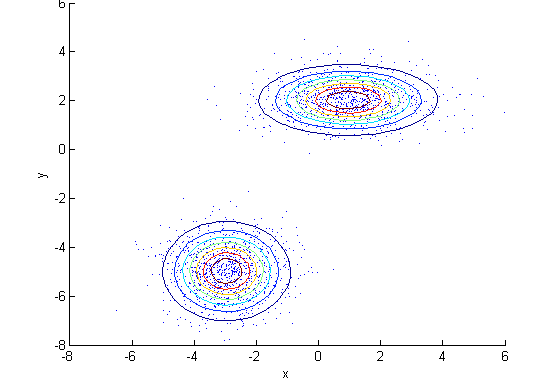
\includegraphics[width=0.50\textwidth]{ourGmmK2.png} &
		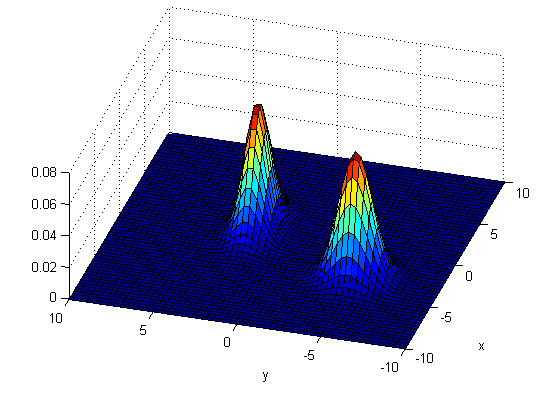
\includegraphics[width=0.50\textwidth]{ourGmmK2-ezsurf.png} \\
	\end{tabular}
	\caption{\label{fig:gmmd2k2}
		Example of GMM with $k=2$, estimated on 2000 points of dimension $d=2$.  }
\end{figure*}


\bibliographystyle{elsarticle-num}
\bibliography{bibliography}
\end{document}
